\section{Problem Set Up} \label{PROBLEM_SETUP}
In this section, we formally introduce the models for which we are estimating parameters: the Lotka-Volterra model and the Shtylla et al. 2019 T1D model \cite{shtylla2019mathematical}. To this effect, we outline the equations of the models and examine experimental data in Section \ref{Model_Desc}. We then discuss how the performance of parameterization techniques on these models can be evaluated and compared in Section \ref{Methodology}. \par We will be returning to the information described in both of these sections as we move through our parameter estimation tutorials starting with MCMC methods, then moving to PSO, and concluding with Kalman Filters. By estimating parameters for these two different ODE systems, one simple, the other complex, we hope to introduce the reader to the mathematics and theory behind each algorithm and illuminate the work of fine-tuning each algorithm implementation to both models. 

\subsection{Model Descriptions} \label{Model_Desc}
\par Two models were used: one a classical, simple example of a dynamical system, and the other a more complicated example from current literature. The simple system in Section \ref{Lotka_Volterra_System} serves solely as a vehicle for a clear and understandable tutorial, while the more complex system in Section \ref{Type1_Diabetes_System} demonstrates a realistic use case for these paramaterization techniques that would arise in biological research. 

\subsubsection{Lokta-Volterra Model} \label{Lotka_Volterra_System}
Natural oscillations have long been observed between predator and prey populations. The Lotka-Volterra model of predator-prey dynamics, developed independently by Alfred J. Lotka and Vito Volterra in the 1920s, is a well-known pair of nonlinear ordinary differential equations that describe these oscillations. It is an elementary example of a dynamical system and will be used as our simple, tutorial system.
\par In the Lotka-Volterra system, the predator population $l$, and the prey population $h$ at time $t$ are given by
\begin{equation} \label{eq:1prob}
\frac{dh}{dt} = \alpha h - \beta hl  \\
\end{equation}
\begin{equation} \label{eq:2prob}
\frac{dl}{dt} = -\gamma l + \delta hl \\
\end{equation}
where $\alpha$ is the intrinsic rate of prey population increase, $\beta$ the rate of predation, $\gamma$ the natural mortality rate of the predator population, and $\delta$ the reproduction rate of the predator population per prey consumed. All parameters take on a single, constant value for the entire data set.
\par This model rests on several simplifying assumptions. First, they prey population will grow exponentially in the absence of the predator population. Second, the predator population will starve in the absence of prey. Finally, there is not a limit to the number of prey that can be consumed by the predator population.
\par In its stable state, each population oscillates with a constant period between a maximum and minimum population, with the peak of the predator's oscillation lagging behind that of the prey's \cite{Lotka} \cite{Volterra}. 

\paragraph{Data}
One of the hallmark data sets in ecology, the Canadian lynx and snowshoe hare pelt-trading records of The Hudson Bay Company provide a classical example of behavior that fits well to the Lotka-Volterra model. Expressed in thousands of individuals, the number of pelts collected from each species was recorded yearly for years 1845-1935 \cite{predpreyHudsonBay}. This quantity acts as a proxy for population. We concede that this data does not represent as perfect Lotka-Volterra system: the populations reached by each species year-over-year are not the same, and the timing of peaks is not always consistent with the predator-prey lag predicted. However, since simplicity is important to our tutorial, we deem the Lotka-Volterra model reasonable for our purposes. 

\begin{figure}[H]
    \centering
    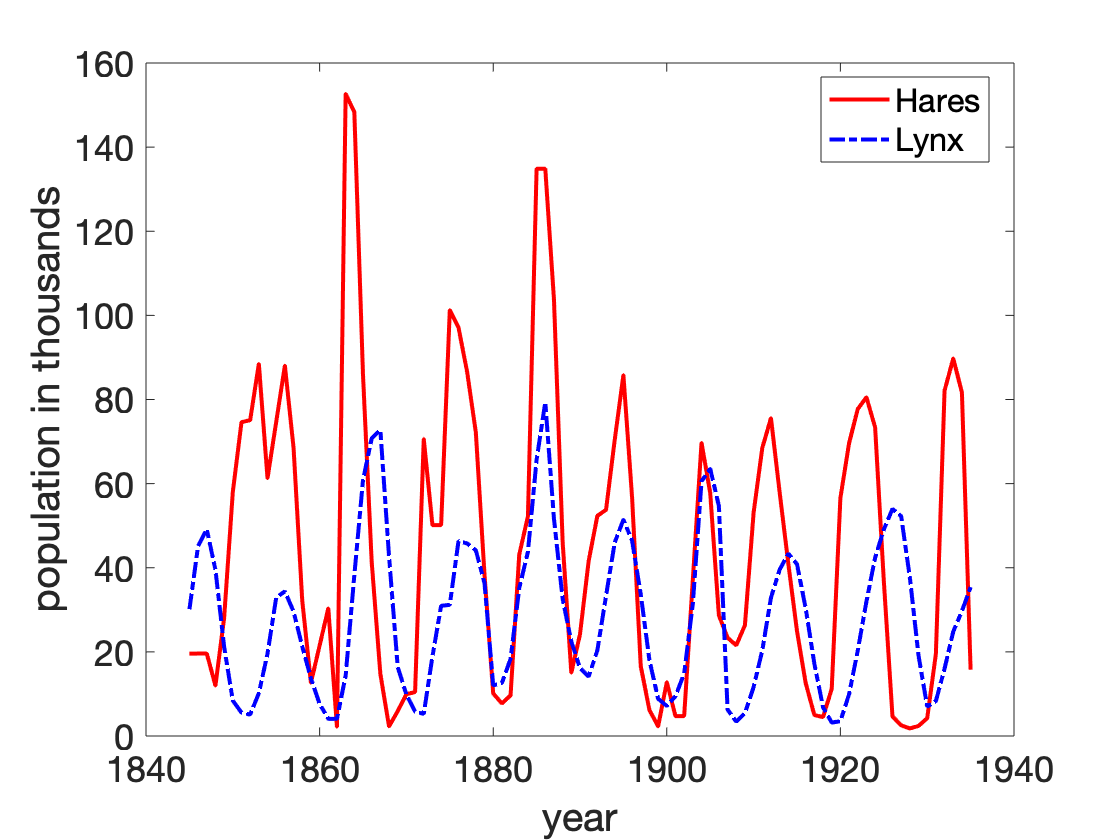
\includegraphics[width=15cm]{Model_Setup_Images/HaresLynxData.png}
    \caption{Hare-Lynx populations (in thousands) as determined by the pelt records of the Hudson Bay Company from 1845-1935. Note the oscillations between the populations, the hallmark of the Lotka-Volterra model.}
    \label{fig:0prob}
\end{figure}

\paragraph{Quantities of Interest} \label{section:LV_params}
All model parameters: $\alpha, \beta, \gamma, \delta$, are considered to be unknown. This makes them quantities of interest for estimation through MCMC, PSO, and Kalman Filtering. Additionally, an amount of noise exists within the data. The approach to account for this noise during paramterization is different between the parameterization techniques. In MCMC, noise is estimated iteratively as is detailed in Section \ref{Metropolis_MCMC}. In Kalman Filters, an estimate for the amount of Gaussian noise is made prior to the filtering process (detailed in Section \ref{noise_UKF}). Alternatively, in PSO we seek to estimate the amount of noise in the data \emph{during} the parameterization routine. This is done by treating the variance of noise for each species as an additional parameter: $\sigma^{2}_{H}$ and $\sigma^{2}_{L}$, for hares and lynx respectively. This assumes that the noise, $\epsilon$, within the two populations is independent. $\sigma^{2}$ represents the variance of this noise, assuming Gaussian noise centered around 0,
\begin{center}
$\epsilon_{h}\sim\mathcal{N}(0,\sigma_{h}^{2})$\\
$\epsilon_{l}\sim\mathcal{N}(0,\sigma_{l}^{2})$
\end{center}
In total, six parameters were estimated for in PSO, and four in both MCMC and Kalman Filtering. Denoting the parameter set by $\theta$,
$$\theta = [\alpha, \beta, \gamma, \delta, \sigma_{H}^{2}, \sigma_{L}^{2}]$$ for PSO, and $$\theta = [\alpha, \beta, \gamma, \delta]$$ for MCMC and the UKF.

\paragraph{Initial parameter guess} \label{section:LV_initParams}
In our implementations, MCMC and Kalman filters both require a user-defined initial guess for the values of the parameters. Notably, our implementation of PSO did not require a user-defined guess, but did require bounds to be defined for parameter values as discussed in Section \ref{param_bounds} . The same bounds were required for MCMC.
\par An initial parameter guess provides MCMC and the UKF a point from which to start their estimation. In practice, these initial parameters can be decided using a variety of means. However, a better initial parameter guess causes faster convergence to the ideal parameters determined by each algorithm.
Based on other parameterization work done on the Hudson Bay Company data set \cite{predpreyHudsonBay}, we initially guessed values $\alpha = \gamma = 0.7$ and $\beta = \delta = 0.1$, though we had no reference for the viability of these parameters. 
\par Due to our uncertainty, this guess was then improved by a running a preliminary \emph{unconstrained nonlinear optimization} routine with MATLAB's default \texttt{fmincon} (documentation found \textit{\href{https://www.mathworks.com/help/optim/ug/fmincon.html}{here}}) \cite{MATLAB:2020b}. Unconstrained nonlinear optimization is a common, fast, and relatively simple technique for parameter fitting \cite{Simunek2002nonlinearfitting} \cite{optimizationparamest_ppt}. By reducing the sum-of-squares difference between the model output and the data to a desired tolerance, a 'best-fit' set of parameters is chosen. While \texttt{fmincon} provides a good preliminary parameter estimate, MCMC and Kalman Filtering can be used to tune these parameters further, potentially resulting in a better fit. The resultant parameter set $\theta_{min}$ for MCMC and the UKF is 
\begin{center}
    $\theta_{min} = [0.625, 0.190, 0.661, 0.0468]$
\end{center}. 
This was taken to be the initial parameter guess.

\paragraph{Parameter bounds} \label{param_bounds}
Upper and lower bounds for the values of each parameter needed to be defined for both MCMC and PSO. In the general case, these bounds can be informed by reasonable, physical limits on the parameters (i.e. parameter $x$ must be non-negative), however when this information is not available, parameters are commonly let to vary a certain percentage above and below their initial value. Using the initial parameter guess for MCMC, values were allowed to range $\pm 100\%$. For the $\sigma_{H}^{2}$ and $\sigma_{L}^{2}$ values required by PSO but left undefined by $\theta_{min}$, ranges were defined using initial estimates for the variances. Residuals between the data and the model predictions solved using $\theta_{min}$ as defined above were found. Then, variances of these residuals was calculated to give
$${\sigma_{H}^{2}}_{initial} = 1487.277$$
$${\sigma_{L}^{2}}_{initial}  = 268.840$$
These values, like those in $\theta_{min}$, were also allowed to vary $\pm 100\%$, defining the upper and lower bounds.

\subsubsection{Type 1 Diabetes Model} \label{Type1_Diabetes_System}
Contemporary research is being done to model Type 1 diabetes (T1D) with dynamical systems. To demonstrate the utility of MCMC, PSO, and Kalman Filtering for parameter estimation in a realistic research context, one such model is examined.
\par Type 1 diabetes is an autoimmune disease characterized by the inability to regulate blood glucose, leading to chronically elevated glucose levels. These elevated glucose levels are a result of abnormal immune attacks on insulin-producing $\beta$-cells within the pancreas. Cells in the body respond to insulin by absorbing glucose from the blood, thus lowering blood glucose levels. Therefore, when these $\beta$-cells are damaged, and normal insulin production is disrupted, blood glucose rises to exceed healthy levels. 
\par One is genetically predisposed for Type 1 diabetes, however onset of the disease is theorized to be determined by the immune system's ability to respond to early structural changes in the pancreas, known as the \emph{apoptotic wave}. The apoptotic wave occurs in mammals during weaning when there are high rates of pancreatic $\beta$-cell apoptosis (natural, controlled cell death). As described above, the apoptosis of $\beta$-cells causes glucose levels to rise. Put simply, if blood glucose is able to return to healthy levels after this wave, diabetes onset does not occur. Likewise, if it is not, diabetes onset occurs, and chronically elevated glucose levels follow. The cellular mechanics of this onset are complex and largely uncertain, but hypothetical onset can be modeled with a dynamical system \cite{shtylla2019mathematical}.
\par Shtylla et al. details a single compartment model that models macrophage, immune cell, and dendritic cell populations within the pancreas, as well as blood insulin and glucose levels for genetically-engineered non-obese diabetic (NOD) mice. The 12-equation nonlinear ODE model includes 53 biologically-driven parameters, such as the volume of blood in the pancreas, the clearance rate of various macrophages, and the basal rate of glucose production, to name a few \cite{shtylla2019mathematical}. A description of these parameters and the equations of the model are included in Appendix A. In previous work, parameter values were estimated from biological literature and altered experimentally to resemble average system behavior seen in collected data, however the model was not parameterized directly to observed data.

\begin{figure}[H]
    \centering
    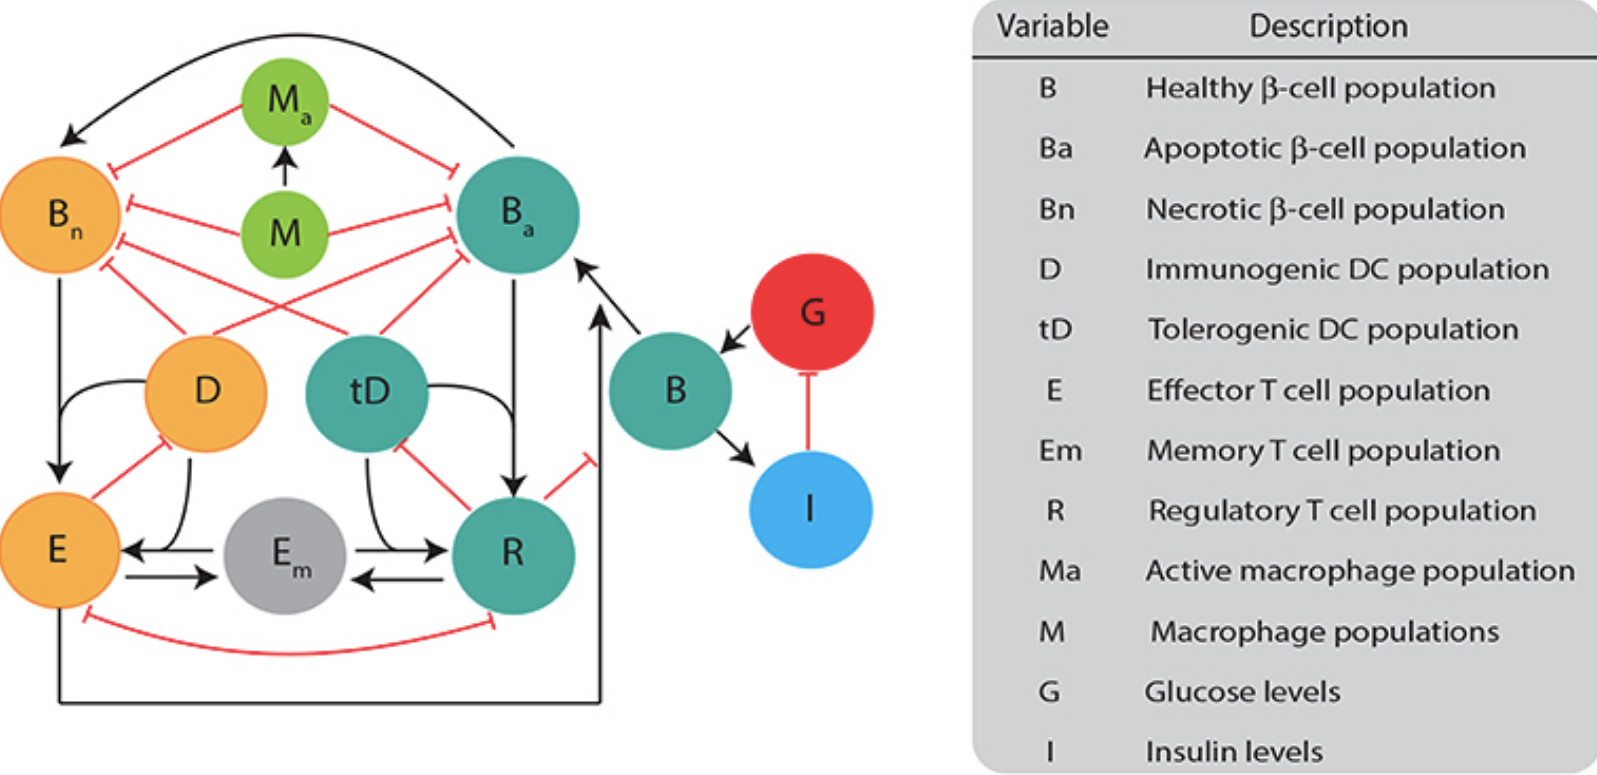
\includegraphics[width=15cm]{Model_Setup_Images/T1Dflowdiag.png}
    \caption{Flow diagram of T1D model in use, taken from Shtylla et al. 2019. As per Shtylla et al., "$\beta-$cell populations are split into three categories: healthy population ($B$), apoptotic cells ($B_{a}$), and necrotic cells ($B_{n}$). Healthy $\beta-$cells are involved in glucose ($G$) and insulin ($I$) regulation, whereas the dying $\beta-$cells (apoptotic and necrotic) interact with immune cells. Dendritic cells are split into two categories: immunogenic DC ($D$) and tolerogenic DC ($tD$) based on their ability to engage an immunogenic or tolerogenic T cell response. DCs in our model are assigned into a particular category once they engulf either apoptotic or necrotic $\beta-$cells. Macrophages can either be in an activated ($M_{a}$) or non activated form ($M$) based on their capacity to engulf $\beta-$cells. T cells are split into: regulatory T ($R$), effector T ($E$), or memory T ($E_{m}$). All populations are measured in cells ml−1 except for $B$ (mg), $G$ (mg/dl), and $I$ ($\mu$U)." \cite{shtylla2019mathematical}}
    \label{fig:flowdiag}
\end{figure}

\paragraph{Data}
While the Lotka-Volterra model functions on a population-level, data provided for the T1D model represents the system for a single mouse. In order to gain insights into the behavior of T1D in both individuals and on a population-level, the observed data used was manipulated to represent the cohort in its entirety. 

\subparagraph{Individual data} \label{section:T1D_individual_data}
Glucose data was measured in a cohort of 11 diabetic NOD mice by Li et al. 2009 \cite{Lietal2009}. In comparison to the 11 other quantities given by the Shtylla et al. model, glucose is easily measurable and a common quantity to keep track of in NOD mice \cite{Mathewsetal2015}. Glucose is also the metric used to diagnose and manage diabetes. Based on biological literature, Type 1 diabetes in NOD mice is diagnosed as having onset at a blood glucose level above 250 mg/dl \cite{Mathewsetal2015}.
\par In this data set and others of the same variety, there appear to be two distinct mouse behaviors: an \emph{acute} rise in glucose prior to onset, and a \emph{progressive} climb. Mice are classified visually and separated by this behavior \cite{Mathewsetal2015}. In the Li et al. data set, 9 mice were classified as acute and 2 as progressive. Our analysis focuses on the 9 acute mice, the raw data for which are included in Appendix \ref{general_appendix}.

\begin{figure}[H]
    \centering
    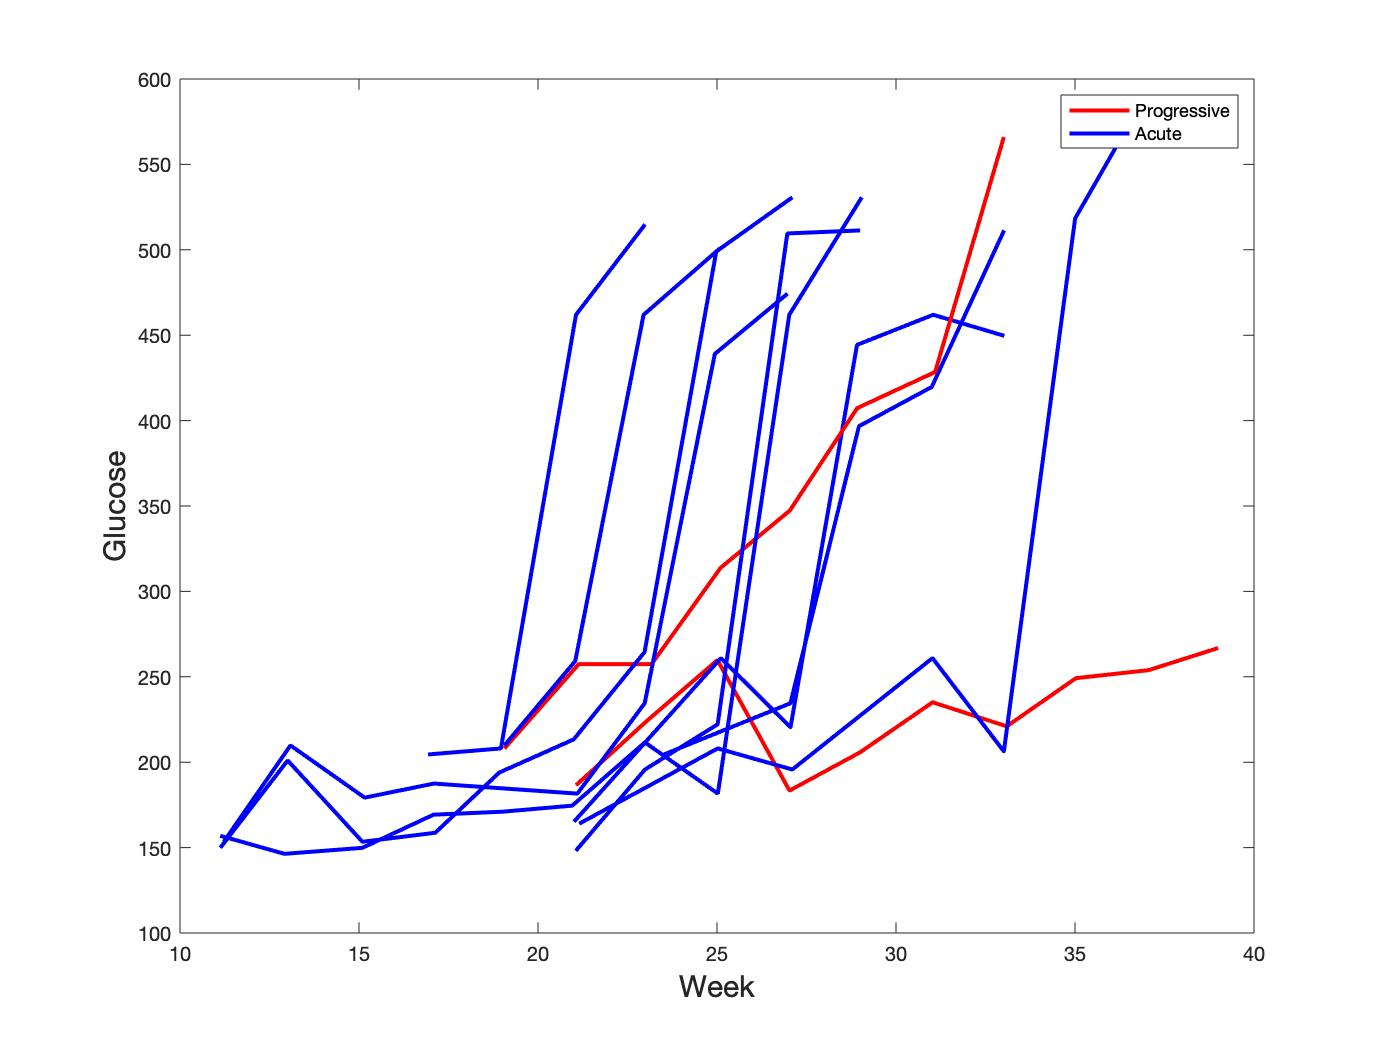
\includegraphics[width=15cm]{Model_Setup_Images/AcuteVersusProgressive.jpg}
    \caption{Glucose levels of the cohort of 11 NOD mice from Li et al.. The 2 mice that experience a progressive rise to diabetes onset are highlighted in red, while the 9 mice experiencing an acute form of onset are in blue.}
    \label{fig:1prob}
\end{figure}

\par In examining the data set itself, measurements are taken at inconsistent time points starting several weeks into each mouse's life. Time was measured in weeks as a decimal to include accuracy down to the time of day when the measurement was taken. On average, measurement started at week 30.47, and measurements were taken every 2.15 weeks. There was also not a consistent number of data points for each mouse in the cohort. Ranging from 4 to 11, the mean number of data points was 6.91. In order to make these somewhat sparse, inconsistently spaced data compatible with the dynamical system, they had to be converted to days. This was simply done by multiplying the associated week value by 7.

\subparagraph{Population-level data} \label{section:T1D_population_data}
We seek to estimate general parameters for diabetes onset in NOD mice, in addition to estimating parameters in a \emph{single} NOD mouse. As addressed within the descriptions of techniques themselves, the different parameterization techniques function differently to fit these population-level parameters. During our experimentation with different data sets, we found that Kalman Filters functioned best with individual mouse data sets due to the way in which the algorithms deal with the noise of the system and data. We also found that MCMC techniques tended to work better with the averaged data, likely due to the fact that MCMC is less concerned with error noise in the data. Thus, as will be explicitly explained in subsequent sections, the Kalman Filters use results from fitting each mouse individually to estimate population parameters and MCMC uses a population-level data set. PSO can use both approaches.
\par To construct a population-level data set from individuals' data, taking a point-by-point average is an intuitive, common method. However, this was avoided for the Li et al. data set. If averaged, the shape of the glucose curves would largely be lost due the staggering of diabetes onset times in the mouse population. Representing an average mouse would not be well-accomplished with this strategy. Instead, we developed a method to align each individual's glucose curve in time and then average all nine curves to preserve shape. 
\par While not ideal for larger data sets, our main approach was done by hand. We were most interested in the capturing the overall shape of the acute mice onset curve: the slow increase of glucose and the sudden spike indicating diabetes onset. Our approach relies on averaging both the glucose measurements and time spans of each mouse. Generally, we sought to align the 9 mice at the point immediately before the large spike in glucose that denoted onset (typically the 3rd or 4th point from the end), here we will name them \emph{pivot points}. This conserves the shape of the onset curve. \textbf{Figure 
\ref{fig:2prob}} highlights the pivot points within the acute Li et al data.
\begin{figure}[H]
    \centering
    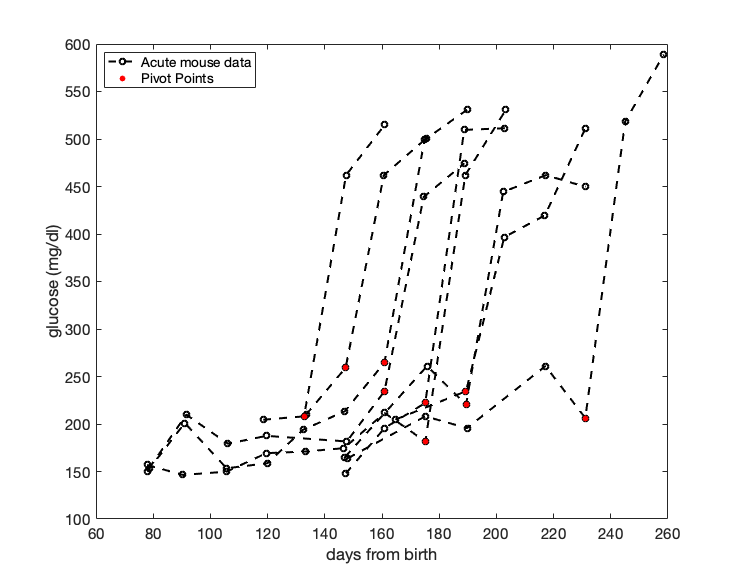
\includegraphics[width=15cm]{Model_Setup_Images/acute_pivotPoints.png}
    \caption{Diagram illustrating the process of determining glucose pivot points for 9 acute mice. Pivot points are indicated in red.}
    \label{fig:2prob}
\end{figure}
\par We began by discretizing the data: by creating an uniformly spaced time span incremented week by week, we could align the data points by absolute week of measurement, leaving weeks where mice were not measured blank. This was done in discrete, whole weeks. In determining which week to which to align each data point, we rounded weeks in the data set to the nearest whole number. For example, a measurement with the time 36.932 was aligned with the 37 week mark, while a time of 27.104 was aligned with the 27 week mark. \textbf{Figure \ref{fig:3prob}} shows this process for Mouse 6.
\begin{figure}[H]
    \centering
    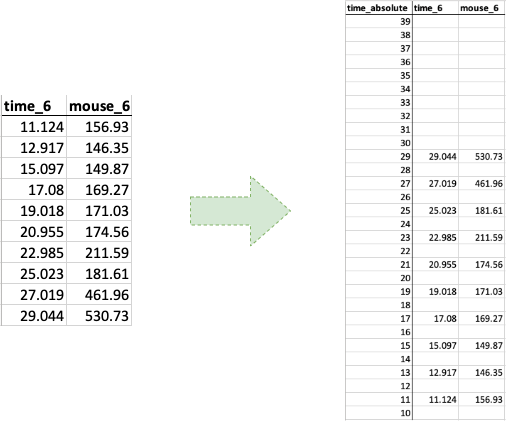
\includegraphics[width=15cm]{MCMC_figs/lietal_avg_diagram.png}
    \caption{Diagram illustrating the process of spacing Mouse 6 data within the 10-38 week time span. Using rounded times, Mouse 6 glucose measurements were spaced in an Excel sheet within the 10-38 week time span. The cells on the left show the original raw data with original time points and the cells on the right show how the original data is spaced within the prescribed 10-38 week time span.}
    \label{fig:3prob}
\end{figure}
The time series then needed to be shifted to align their pivot points before an average could be taken. This shifting simply involved the vertical movement of the time series in the spreadsheet, however the aligned curves must placed at some time along the $x$-axis. Shifting the data removes information about what this time should be. To define the time of pivot, we determined the average time of pivot across the population according to the data, and placed the pivot point accordingly. Times of the other data points were adjusted to maintain the correct spacing. Then, both the nondiscretized time values and the glucose values could be averaged and rounded to 3 significant figures to construct a data set representing the population: that of an average mouse. This process is diagrammed for Mouse 6 in \textbf{Figure \ref{fig:3prob}}. 
\par Lastly, each week value was multiplied by 7 to convert the timescale from weeks to days. The Shtylla et al. model uses days as its time scale, so this conversion makes the data set and the model compatible.
\par \textbf{Figure \ref{fig:4prob}} shows the plot obtained after the shifting and averaging process. As pictured, the sharp spike in glucose observed on the individual level is conserved, avoiding the issues encountered when taking averages. This was taken to be the population-level data set. 
\begin{figure}[H]
    \centering
    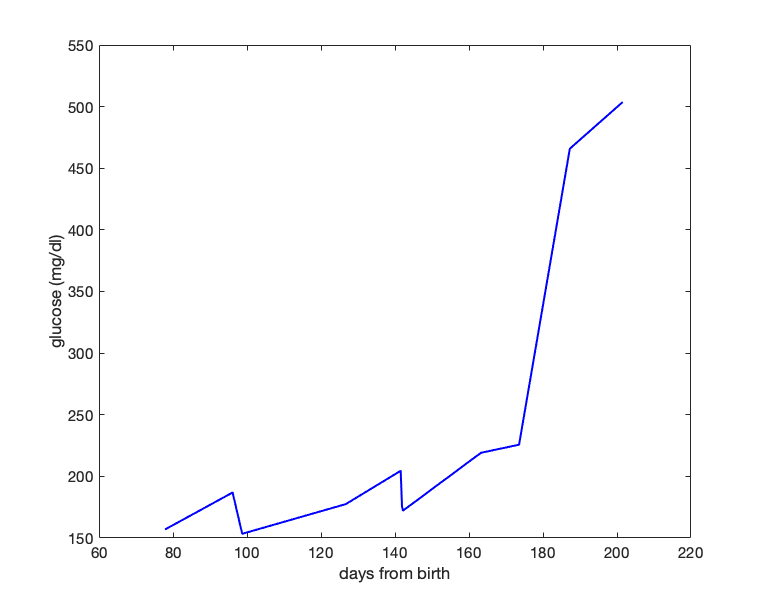
\includegraphics[width=15cm]{Model_Setup_Images/avg_raw_plot.png}
    \caption{Plot of the averaged and shifted acute mouse data. Constructed from 9 individual NOD mice, this was taken to represent the population-level data set.}
    \label{fig:4prob}
\end{figure}
\paragraph{Quantities of Interest}
There are 53 biologically-informed values built into the model, however 12 function as conversion rates, or otherwise known quantities \cite{shtylla2019mathematical}. Since these are known to be constant and pre-defined, they are not included in $\theta$. The remaining 41 values are treated as variable within the system and are quantities of interest for parameter estimation. For more information see Appendix \ref{general_appendix}.
\par To minimize computation and incorporate more certainty about parameters in the system, subsets of these 41 parameters were estimated while other parameters were held relatively constant. By letting some parameters remain relatively constant, we tell our system that we are fairly confident that their values are correct. However, the values are still allows to change in very small ways; 1 percent of their original range. This was done to account for correlations between the parameters. As of yet, sensitivity analysis has not been done to identify correlated parameters, so this step was taken to encourage the natural behavior of related parameters, even within the limited system.
\par These subsets were chosen experimentally. Only one of the tested subsets proved significant, referred to as the \emph{notable parameter subset}. This subset allowed for enough flexibility to find a relatively good fit to data, unlike others tested.
\subparagraph{Notable parameter subset} \label{section:NotableParameterSubset}
The notable parameter subset is composed primarily of 'active' parameters according to the Kalman Filter. 'Active' describes a greater than 1 percent change from the baseline to the fitted value for each parameter when the UKF was run on all the parameters. Upon inspection of the results from Kalman Filtering, few parameters moved beyond this threshold, so these parameters were marked as significant. Seven parameters were marked as active: $G_{I}, S_{I}, \mu_{E}, \mu_{R}, e_{1}, e_{2},$ and $\delta_{B}$.
\par In addition to the active parameters, three other parameters were added to the notable set: $\eta, \alpha_{\eta}, and \beta_{\eta}$, referred to as the $\eta$ parameters. Simply put, these parameters relate to the effectiveness of T-cells at eliminating insulin-producing $\beta$-cells. This heavily impacts the time of diabetes onset, and thus manipulating these parameters allows for horizontal shifting of the fit. While the active parameters influence the shape of the glucose spike more, these $\eta$ parameters allow for greater flexibility in the onset time. Shape and position are the main indicators of fit, and this notable parameter set does a sufficient job of addressing both while lessening computation and building more certainty about parameters within the system. 
\par This subset was required only by MCMC due the need to have more data points than parameters. However, for comparison purposes, the subset was also run in PSO. 

\paragraph{Initial parameter guess}
As parameterization of the model using the methods in this paper is intended to improve upon the findings in Shtylla et al., the biologically estimated parameters and initial conditions from Shtylla et al. were used as an initial guess $\theta$ for the parameters for each technique \cite{shtylla2019mathematical}. 

\subsection{Comparison Methodology} \label{Methodology}
In order to evaluate and compare the effectiveness of each parameterization technique, a method needed to be devised to quantify a model's goodness of fit to a data set. Because the goal of each parameterization technique is to produce system predictions that are close to observed data, this metric needs to measure the distance between the model and the data. Root Mean Squared error (RMSE) was chosen as this metric to quantify the mean residual between the model and the data set at one data point. 
\par RMSE quantifies the standard deviation of residuals, or prediction errors. The prediction error is the distance between the model prediction and the observed data at each time point $t$. RMSE tells us how concentrated the original data points are around our prediction. This was thought to be a more useful technique than simply MSE, or mean squared error, due to the magnitude of the datapoints observed. For more information regarding RMSE see \textit{\href{https://statweb.stanford.edu/~susan/courses/s60/split/node60.html}{here}.}